\chapter{Analyse de l'existant}

\section{Démarche d'analyse de l'existant}

\noindent Pour évaluer le positionnement de \textbf{SecuCom} dans le paysage des solutions destinées aux secrétariats sociaux, une analyse approfondie des plateformes existantes a été menée. Cette démarche s'est articulée autour de plusieurs axes :

\begin{itemize}[leftmargin=*,label=\textcolor{darkgray}{$\bullet$},itemsep=0.3em]
  \item Étude documentaire des solutions leaders du marché belge, notamment via leurs sites officiels, leurs documentations techniques et leurs présentations commerciales
  \item Entretiens avec des utilisateurs actuels de ces plateformes au sein de différents secrétariats sociaux
  \item Analyse comparative des fonctionnalités, des modèles tarifaires et des approches d'intégration
  \item Identification des forces et faiblesses de chaque solution par rapport aux besoins spécifiques des petits secrétariats sociaux comme Sodabel
\end{itemize}

\vspace{0.5cm}

\noindent Cette méthodologie a permis d'établir une cartographie précise de l'offre existante et d'identifier les opportunités pour une solution comme \textbf{SecuCom}. Deux acteurs majeurs ont particulièrement retenu notre attention en raison de leur prédominance sur le marché belge : EasyPay et Liantis.

\begin{note}
L'analyse comparative s'est concentrée sur les fonctionnalités pertinentes pour les petits secrétariats sociaux, en accordant une attention particulière à la facilité d'utilisation, au coût et à l'adéquation avec les processus métier spécifiques de structures comme Sodabel.
\end{note}

\section{Analyse comparée des solutions}

\subsection{EasyPay}

\begin{figure}[H]
    \centering
    
\includegraphics[width=0.5\textwidth]{easyPayLogo.jpeg}
    \caption{Logo d'EasyPay Group \cite{easypay}}
    \label{fig:easyPayLogo}
\end{figure}

\noindent EasyPay Group se positionne comme un acteur incontournable dans le domaine des services de secrétariat social et de gestion des ressources humaines en Belgique. Cette plateforme propose une suite complète d'outils couvrant l'ensemble des besoins administratifs et RH d'une entreprise :

\begin{itemize}[leftmargin=*,label=\textcolor{darkgray}{$\bullet$},itemsep=0.3em]
  \item Gestion complète de la paie et des déclarations sociales
  \item Administration du personnel de A à Z
  \item Gestion des temps et des plannings
  \item Recrutement et sélection
  \item Développement des compétences et formations
  \item Outils de reporting et tableaux de bord RH
  \item Solutions de digitalisation des processus RH
\end{itemize}

\vspace{0.5cm}

\noindent L'écosystème EasyPay se caractérise par sa richesse fonctionnelle et son approche intégrée. Chaque module communique avec les autres, offrant une expérience utilisateur cohérente et des flux de données optimisés. Cette intégration poussée représente un avantage considérable pour les grandes structures ayant des besoins diversifiés.

\begin{figure}[H]
    \centering
    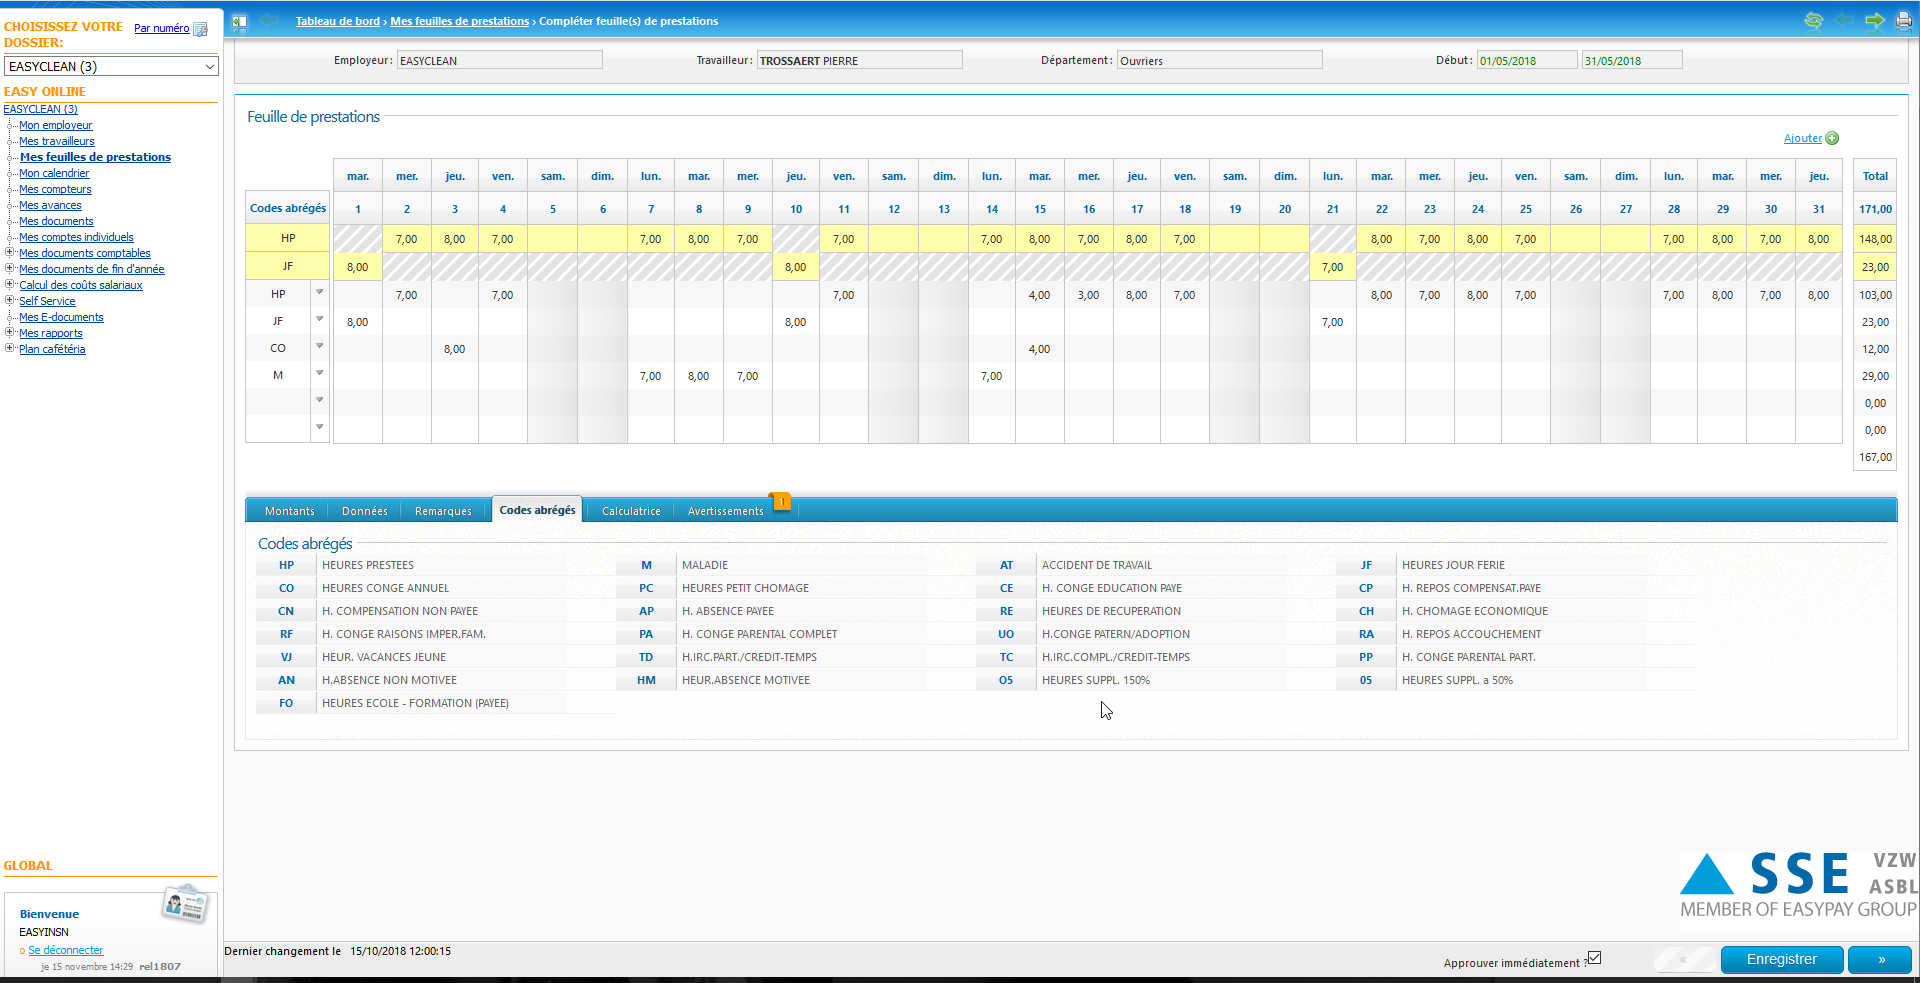
\includegraphics[width=0.9\textwidth]{easyPayScreenshot.png}
    \caption{Capture d'écran de l'interface d'EasyPay \cite{easypay}}
    \label{fig:easyPayScreenshot}
\end{figure}

\begin{tcolorbox}[
  title={\textbf{Limites d'EasyPay pour les petites structures}},
  colback=blue!5!white,
  colframe=primarycolor,
  fonttitle=\bfseries,
  boxrule=0.5mm,
  arc=2mm,
  left=6mm,
  right=6mm,
  top=6mm,
  bottom=6mm
]
\noindent Cette exhaustivité constitue également le principal inconvénient d'EasyPay pour les petites structures comme Sodabel. La plateforme s'avère souvent :
\begin{itemize}[leftmargin=*,label=\textcolor{darkgray}{$\bullet$},itemsep=0.3em]
  \item Excessivement complexe à appréhender et à maîtriser
  \item Coûteuse à déployer et à maintenir
  \item Surdimensionnée par rapport aux besoins réels d'un petit secrétariat social
  \item Rigide dans ses processus, laissant peu de place à la personnalisation fine
\end{itemize}
\end{tcolorbox}

\vspace{0.5cm}

\noindent En outre, bien qu'EasyPay propose des fonctionnalités de gestion des entreprises clientes et de leurs collaborateurs, son interface n'est pas spécifiquement optimisée pour les flux de travail propres aux petits secrétariats sociaux indépendants, qui nécessitent souvent plus d'agilité et de flexibilité dans leurs processus.

\subsection{Liantis}

\begin{figure}[H]
    \centering
    
\includegraphics[width=0.5\textwidth]{liantisLogo.png}
    \caption{Logo de Liantis \cite{liantis}}
    \label{fig:liantisLogo}
\end{figure}

\noindent Liantis représente un autre mastodonte du secteur, né de la fusion de plusieurs acteurs historiques du marché belge. Cette plateforme se distingue par son approche "guichet unique" pour les entrepreneurs et les employeurs, couvrant un spectre extrêmement large de services :

\begin{itemize}[leftmargin=*,label=\textcolor{darkgray}{$\bullet$},itemsep=0.3em]
  \item Secrétariat social complet
  \item Assurances sociales pour indépendants
  \item Médecine du travail et prévention
  \item Allocations familiales
  \item Assurances diverses (accidents du travail, revenu garanti, etc.)
  \item Conseil juridique et accompagnement
  \item Formation et développement
\end{itemize}

\vspace{0.5cm}

\noindent La force de Liantis réside dans cette approche holistique qui permet à une entreprise de gérer l'ensemble de ses obligations sociales et administratives via un seul partenaire. La plateforme offre également des outils numériques modernes et une présence physique étendue à travers la Belgique.

\begin{figure}[H]
    \centering
    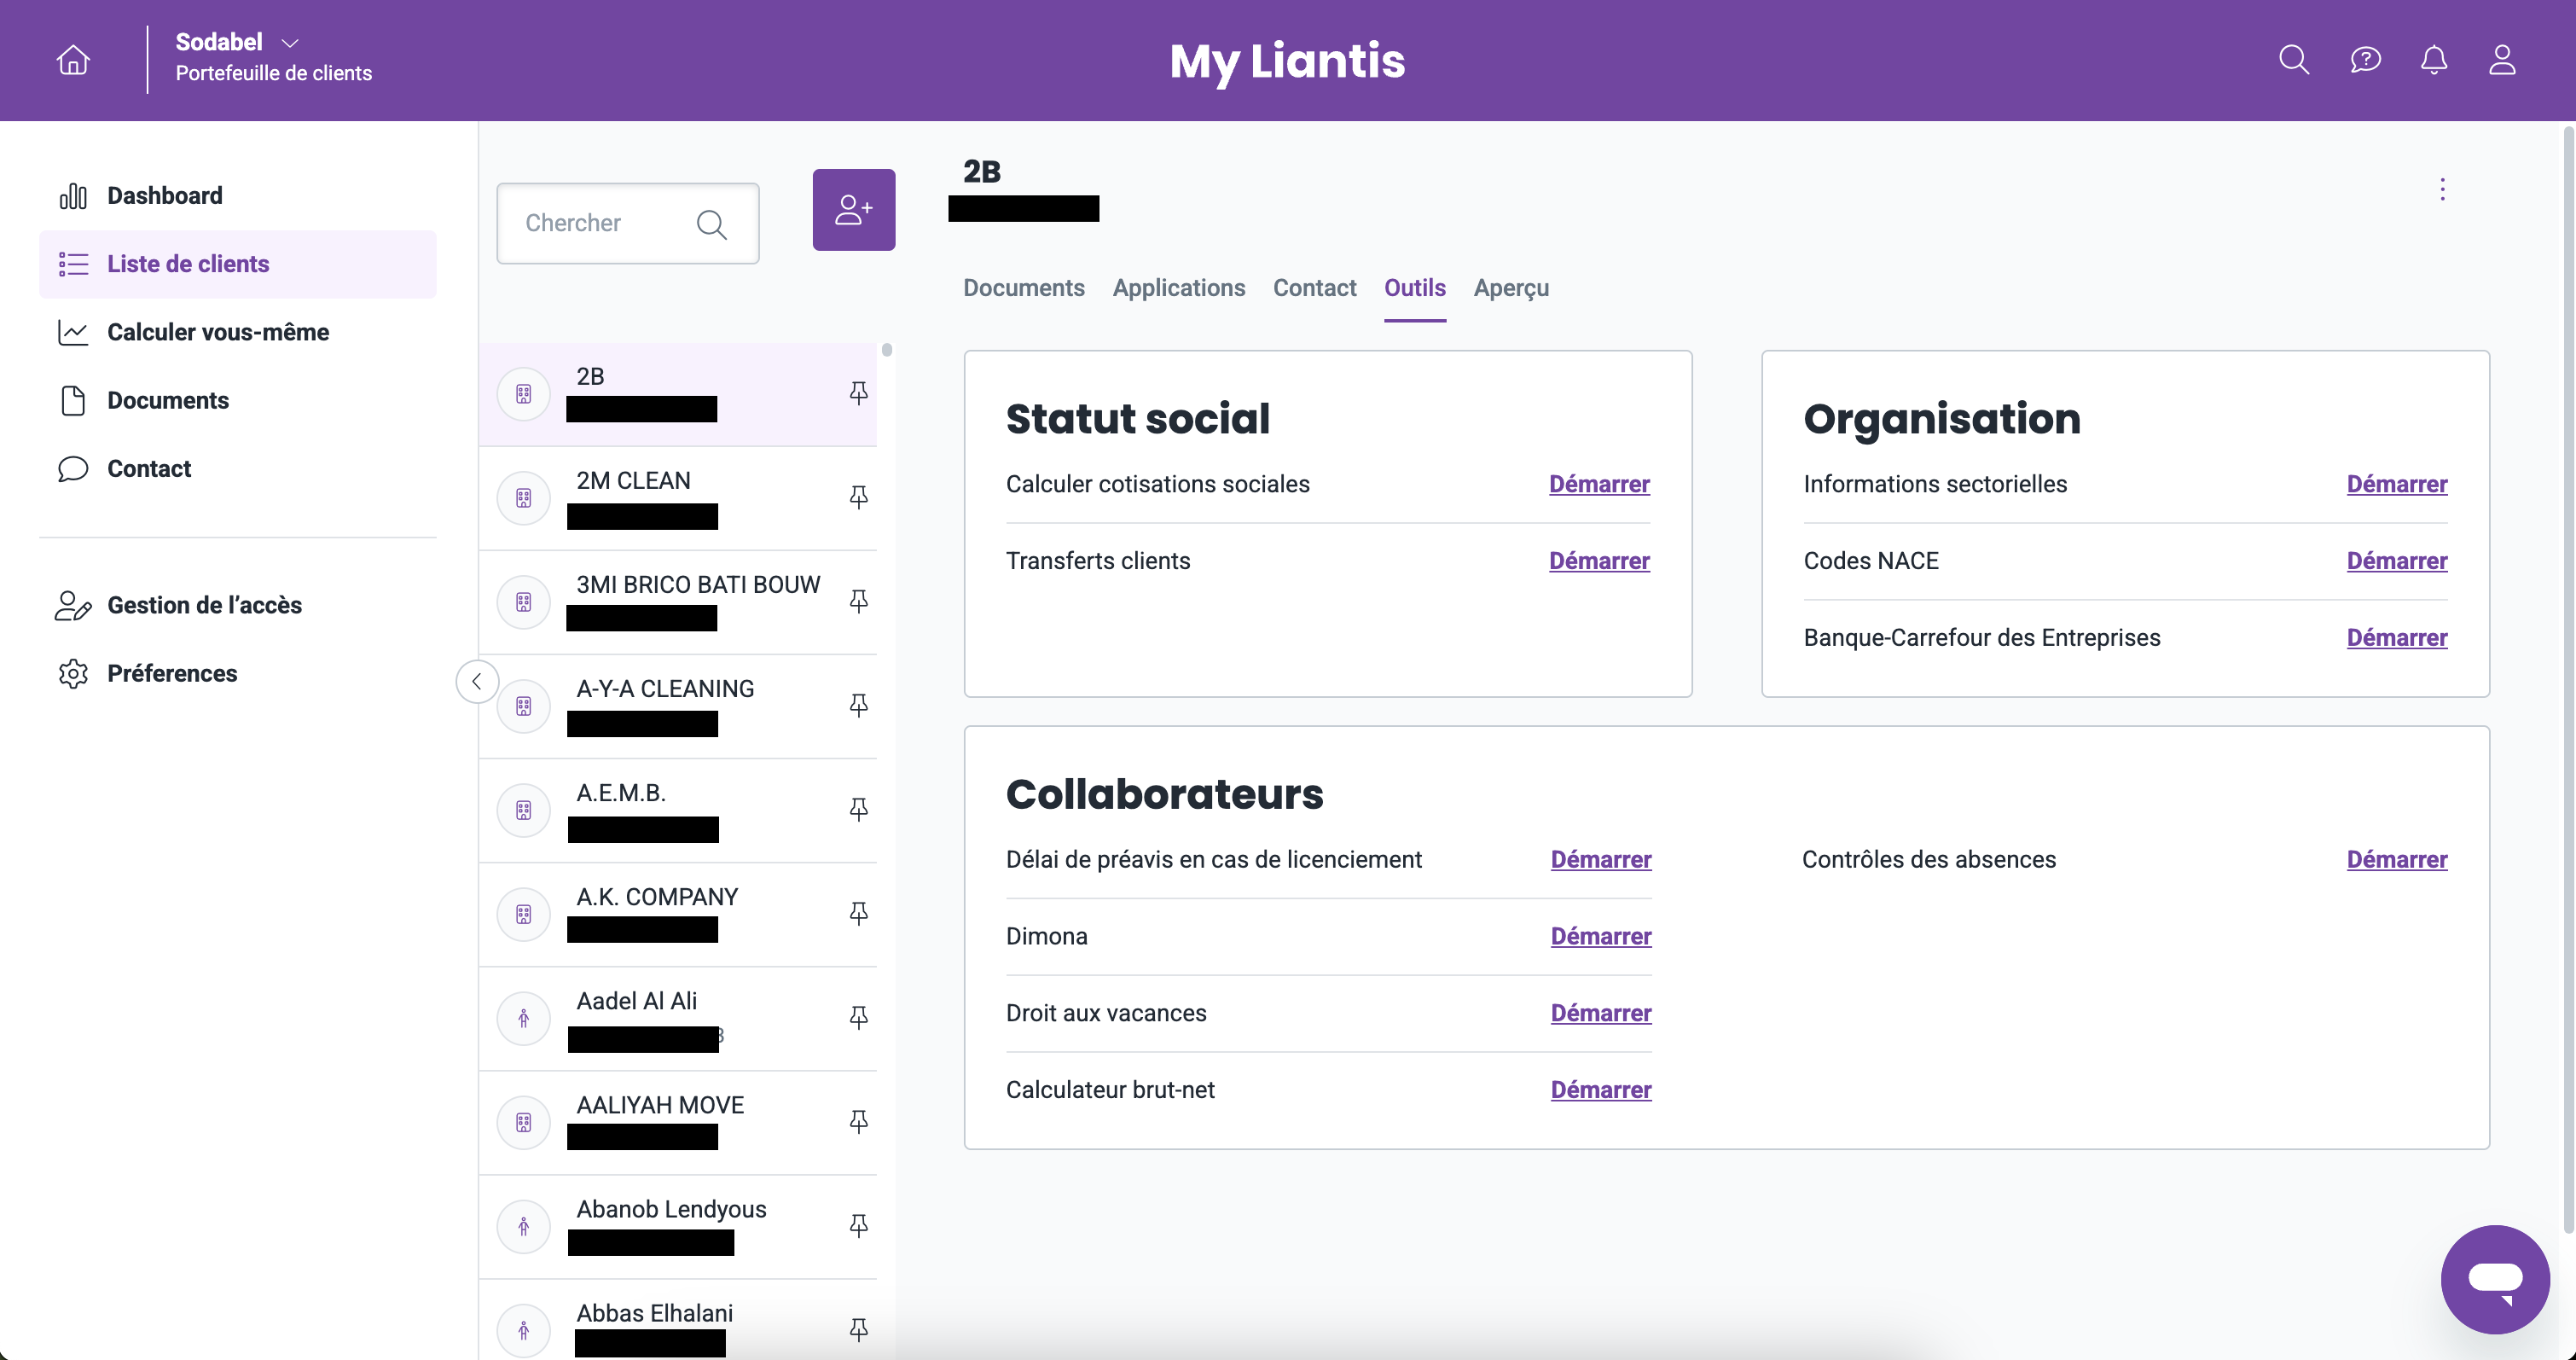
\includegraphics[width=0.9\textwidth]{liantisScreenshot.png}
    \caption{Capture d'écran de l'interface de Liantis \cite{liantis}}
    \label{fig:liantisScreenshot}
\end{figure}

\begin{tcolorbox}[
  title={\textbf{Contraintes de Liantis pour les petites structures}},
  colback=blue!5!white,
  colframe=primarycolor,
  fonttitle=\bfseries,
  boxrule=0.5mm,
  arc=2mm,
  left=6mm,
  right=6mm,
  top=6mm,
  bottom=6mm
]
\noindent Toutefois, comme pour EasyPay, cette exhaustivité s'accompagne de contraintes significatives :
\begin{itemize}[leftmargin=*,label=\textcolor{darkgray}{$\bullet$},itemsep=0.3em]
  \item Une structure tarifaire complexe et souvent onéreuse pour les petites structures
  \item Une certaine lourdeur administrative inhérente à la taille de l'organisation
  \item Des processus standardisés qui peuvent manquer de souplesse
  \item Une interface utilisateur qui, bien que moderne, doit accommoder tant de fonctionnalités qu'elle en devient parfois confuse
\end{itemize}
\end{tcolorbox}

\vspace{0.5cm}

\noindent Par ailleurs, la spécialisation de Liantis dans tant de domaines différents dilue inévitablement son focus sur les besoins spécifiques des petits secrétariats sociaux en matière de gestion des entreprises clientes et de leurs collaborateurs.

\section{SecuCom face à l'existant}

\noindent \textbf{SecuCom} se distingue fondamentalement d'EasyPay et Liantis par son approche ciblée et minimaliste. Là où ces mastodontes tentent de couvrir l'intégralité du spectre des besoins administratifs et sociaux, \textbf{SecuCom} se concentre exclusivement sur l'optimisation des processus de gestion des entreprises clientes, de leurs collaborateurs et des déclarations DIMONA.

\begin{note}
Cette spécialisation délibérée constitue la principale force de \textbf{SecuCom} et répond à un besoin précis que les solutions généralistes, malgré leur richesse fonctionnelle, peinent à satisfaire efficacement. \textbf{SecuCom} n'a jamais eu l'ambition de rivaliser frontalement avec ces géants du secteur, mais plutôt de combler une niche spécifique avec une solution sur mesure.
\end{note}

\begin{tcolorbox}[
  title={\textbf{Avantages distinctifs de SecuCom}},
  colback=blue!5!white,
  colframe=primarycolor,
  fonttitle=\bfseries,
  boxrule=0.5mm,
  arc=2mm,
  left=6mm,
  right=6mm,
  top=6mm,
  bottom=6mm
]
\noindent Les avantages distinctifs de \textbf{SecuCom} par rapport à ces plateformes généralistes sont multiples :

\begin{itemize}[leftmargin=*,label=\textcolor{darkgray}{$\bullet$},itemsep=0.3em]
  \item \textbf{Simplicité et intuitivité} : Interface épurée, focalisée uniquement sur les fonctionnalités essentielles, sans la surcharge cognitive des plateformes tout-en-un.
  \item \textbf{Coût optimisé} : Structure tarifaire simple et adaptée aux petites structures, sans modules superflus à financer.
  \item \textbf{Flexibilité maximale} : Capacité d'adaptation rapide aux processus spécifiques de chaque secrétariat social, contrairement aux workflows rigides des grandes plateformes.
  \item \textbf{Prise en main immédiate} : Courbe d'apprentissage réduite, permettant une adoption rapide sans formation extensive.
  \item \textbf{Focus sur l'essentiel} : Concentration des ressources de développement sur l'optimisation des fonctionnalités réellement utilisées au quotidien.
\end{itemize}
\end{tcolorbox}

\vspace{0.5cm}

\noindent Le tableau comparatif ci-dessous met en évidence le positionnement de \textbf{SecuCom} face à EasyPay et Liantis sur plusieurs critères clés :

\begin{table}[H]
\caption{Comparaison des solutions pour secrétariats sociaux}
\label{tab:comparaison-solutions}

\makebox[\textwidth][c]{%
\renewcommand{\arraystretch}{1.3}
\begin{tabular}{p{3.2cm}p{4.2cm}p{4.2cm}p{4.2cm}}
\toprule
\rowcolor{darkgray} \textcolor{white}{\textbf{Critère}} & \textcolor{white}{\textbf{SecuCom}} & \textcolor{white}{\textbf{EasyPay}} & \textcolor{white}{\textbf{Liantis}} \\
\midrule

\textbf{Étendue fonc\-tionnelle} & 
\textbf{Ciblée} \newline
\small{Gestion entreprises, collaborateurs,\ DIMONA} & 
\textbf{Complète} \newline
\small{Paie, RH, temps, recrutement, etc.} & 
\textbf{Très large} \newline
\small{Social, assurances, médecine du travail, etc.} \\
\midrule

\textbf{Complexité d'utilisation} & 
\textcolor{green!70!black}{\small\textbf{Faible}} \newline
\small{Interface minimaliste} & 
\textcolor{orange!70!black}{\small\textbf{Élevée}} \newline
\small{Nombreux modules interconnectés} & 
\textcolor{red!70!black}{\small\textbf{Très élevée}} \newline
\small{Écosystème complet} \\
\midrule

\textbf{Coût relatif} & 
\textcolor{green!70!black}{\small\textbf{Optimisé}} \newline
\small{Adapté aux petites structures} & 
\textcolor{orange!70!black}{\small\textbf{Élevé}} \newline
\small{Licence + modules} & 
\textcolor{red!70!black}{\small\textbf{Très élevé}} \newline
\small{Services multiples} \\
\midrule

\textbf{Personnalisation} & 
\textcolor{green!70!black}{\small\textbf{Élevée}} \newline
\small{Adaptable aux processus spécifiques} & 
\textcolor{orange!70!black}{\small\textbf{Moyenne}} \newline
\small{Paramétrage dans cadre défini} & 
\textcolor{red!70!black}{\small\textbf{Faible}} \newline
\small{Processus standardisés} \\
\midrule

\textbf{Temps de prise en main} & 
\textcolor{green!70!black}{\small\textbf{Court}} \newline
\small{Quelques heures} & 
\textcolor{orange!70!black}{\small\textbf{Long}} \newline
\small{Plusieurs jours} & 
\textcolor{red!70!black}{\small\textbf{Très long}} \newline
\small{Plusieurs semaines} \\
\midrule

\textbf{Cible principale} & 
\textbf{Petits secrétariats sociaux} \newline
\small{Structures indépendantes} & 
\textbf{Moyennes et grandes entreprises} \newline
\small{Besoins diversifiés} & 
\textbf{Tout type d'entreprise} \newline
\small{Et d'indépendant} \\
\bottomrule
\end{tabular}%
}
\end{table}

\vspace{0.5cm}

\noindent En définitive, \textbf{SecuCom} ne cherche pas à remplacer des plateformes comme EasyPay ou Liantis, mais à offrir une alternative ciblée pour les secrétariats sociaux qui privilégient la simplicité, l'efficacité et la spécialisation. Dans un marché dominé par des solutions toujours plus complètes mais aussi plus complexes, \textbf{SecuCom} répond à un besoin croissant de retour à l'essentiel et d'outils parfaitement adaptés à des cas d'usage spécifiques.

\begin{note}
Cette approche s'inscrit dans une tendance plus large observée dans de nombreux secteurs technologiques : face aux suites logicielles massives qui tentent de tout faire, émergent des solutions spécialisées qui excellent dans un domaine précis. \textbf{SecuCom} incarne cette philosophie dans le secteur des secrétariats sociaux belges.
\end{note}

\begin{tcolorbox}[
  title={\textbf{Évolutivité de SecuCom}},
  colback=blue!5!white,
  colframe=primarycolor,
  fonttitle=\bfseries,
  boxrule=0.5mm,
  arc=2mm,
  left=6mm,
  right=6mm,
  top=6mm,
  bottom=6mm
]
\noindent Il est important de souligner que \textbf{SecuCom} est conçu comme une plateforme évolutive. Bien que la version actuelle se concentre sur les fonctionnalités essentielles de gestion des entreprises, des collaborateurs et des déclarations DIMONA, le projet prévoit des phases d'évolution futures. Ces développements ultérieurs permettront d'enrichir progressivement l'application avec des fonctionnalités additionnelles, tout en préservant sa philosophie de simplicité et d'efficacité. Cette approche modulaire et incrémentale garantit que \textbf{SecuCom} pourra s'adapter aux besoins émergents de ses utilisateurs sans jamais tomber dans le piège de la surcharge fonctionnelle qui caractérise les solutions généralistes.
\end{tcolorbox}
